\lesson{Acid and Base Properties of Salts}
A \textbf{salt} is simply another name for an ionic compound. Different salts can produce ions that
can act as acids or bases, or \textbf{neither}.

\subsection{Salts that Produce Neutral Salts}
In general, \textbf{strong acids and strong bases} have no effect on the pH. This is due
to the strong acid having a weak affinity for hydronium ions (hence it can fully dissociate)
and the strong base not being able to attract the hydronium ions.\\

The conjugate base of a strong acid has virtually no affinity for protons when compared to the
affinity of water molecules; this is why strong acids completely dissociate in aqueous solutions.\\

For instance, the conjugate bases $\ch{Cl^-_{(aq)}}$ and $\ch{NO3^-_{(aq)}}$ (from strong acids) 
do not combine with the $\ch{H3O^+_{(aq)}}$, and as a result, have no effect on the pH.
In other words, strong acids have no effect on the pH.\\

Cations such as $\ch{K^+_{(aq)}}$ and $\ch{Na^+_{(aq)}}$ (from strong bases) have no affinity
for $\ch{H^+_{(aq)}}$ nor can they produce $\ch{H^+_{(aq)}}$. They have no effect on pH either.
In other words, strong bases have no effect on the pH.\\

Since in both cases there is no change in the number of $\ch{H3O^+_{(aq)}}$ ions, there will
be no shift in equilibrium of $\ch{H2O_{(\ell)}}\rightleftharpoons \ch{H3O^+_{(aq)}}+\ch{OH^-_{(aq)}}$,
thus no change in $\ch{OH^-_{(aq)}}$ concentration is observed either.

\begin{important}
    Salts that consist of the cations of strong bases and the anions of strong acids have no 
    effect on the pH of a solution whose solvent is water.
\end{important}

\subsection{Salts that Produce Basic Solutions}
For any salt whose cation has neutral properties and whose anion is the conjugate base of a weak
acid produces a basic solution.\\

For instance, in an aqueous solution of sodium acetate, $\ch{NaCH3COO_{(aq)}}$, the major
species are $\ch{Na^+_{(aq)}}$, $\ch{CH3COO^-_{(aq)}}$, and $\ch{H2O_{(\ell)}}$. As previously
discussed, the $\ch{Na^+_{(aq)}}$ ions has neither acid nor base properties. The acetate ion
however is the conjugate base of acetic acid, a weak acid. This means that the acetate ion has a 
strong affinity for hydronium ions and is a base. Therefore, the acetate ions will react with
the hydrogen in the hydronium ions, causing a shift in the water equilibrium, producing more 
$\ch{OH^-_{(aq)}}$ ions. Hence, the solution becomes basic.

\subsection{Salts that Produce Acidic Conditions}
Salts whose cations are the conjugate acid of a weak base (and whose anions come from a strong
acid) produce acidic conditions.\\

For instance
\[
    \ch{NH4OH}+\ch{HCl}\to \ch{H2O}+\ch{NH4Cl}
\]
The $\ch{NH4Cl}$ will dissociate further with the water molecules. Since $\ch{Cl^-}$ is a strong
acid, it has no affinity for protons. However, ammonia does
\[
    \ch{NH4^+_{(aq)}}+\ch{H2O_{(\ell)}}\rightleftharpoons \ch{NH3_{(aq)}}+\ch{H3O^+_{(aq)}}
\]
Since $\ch{NH4^+_{(aq)}}$ is a weak acid, it gives away protons and hence produces more hydronium
ions. Therefore, the solution becomes acidic.

\subsection{Salts that May be Acidic or Basic}
There are salts where \textbf{both} the cation and anion affect the pH of the solution. For instance,
ammonium acetate $\ch{NH4C2H3O2_{(aq)}}$. In such situations, we will only look at them 
\textbf{qualitatively} and predict whether the solution will be acidic, basic, or neutral.
\begin{bulleted-list}
    \item If $K_a>K_b$, the solution will be acidic
    \item If $K_a<K_b$, the solution will be basic
    \item If $K_a=K_b$, the solution will be neutral
\end{bulleted-list}

\subsection{Hydrolysis of Metal and Nonmetal Oxides}
Metal and nonmetal oxides have low solubility in water. Therefore, we consider their \textbf{reaction}
instead of dissociation in water instead. These reactions produce either acidic or basic solutions
\begin{bulleted-list}
    \item Metal oxides react with water to produce basic solutions
    \item Nonmetal oxides react with water to produce acidic solutions
\end{bulleted-list}

For instance, the reaction of the metal oxide calcium oxide in water
\[
    \ch{CaO_{(s)}}+\ch{H2O_{(\ell)}}\to \ch{Ca^{2+}_{(aq)}}+\ch{2OH^-_{(aq)}}
\]
Where the oxide ions are believed to react with the water to form hydroxide ions, thus producing
a basic solution
\[
    \ch{O^{2-}_{(s)}}+\ch{H2O_{(\ell)}}\to \ch{2OH^-_{(aq)}}
\]
Another example is with carbon dioxide, a nonmetal oxide
\begin{align*}
    \ch{CO2_{(g)}}+\ch{H2O_{(\ell)}}&\rightleftharpoons \ch{H2CO3_{(aq)}}\\
    \ch{H2CO3_{(aq)}}+\ch{H2O_{(\ell)}}&\rightleftharpoons \ch{H3O^+_{(aq)}}+\ch{HCO3^-_{(aq)}}
\end{align*}
The $\ch{H2CO3_{(aq)}}$ cancel out and the net equation is
\[
    \ch{CO2_{(g)}}+\ch{2H2O_{(\ell)}}\rightleftharpoons \ch{H3O^+_{(aq)}}+\ch{HCO3^-_{(aq)}}
\]
Producing an acidic solution.

\subsection{Lewis Acids and Bases}
\begin{bulleted-list}
    \item \textbf{Lewis acid:} an atom, ion, or molecule that is an \textbf{electron-pair} acceptor
    \item \textbf{Lewis base:} an atom, ion, or molecule that is an \textbf{electron-pair} donor
\end{bulleted-list}

\begin{figure}[ht!]
    \centering
    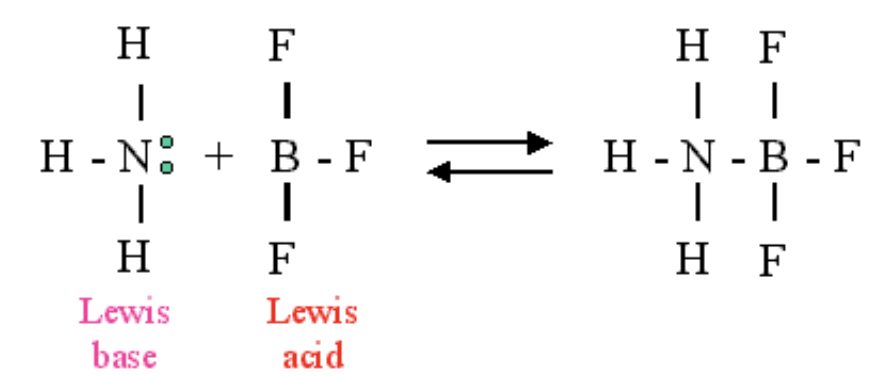
\includegraphics[width=0.5 \textwidth]{../figures/lewis-acid-and-base.png}
\end{figure}
